\section{Diagramme}


Bevor wir mit der Implementation des Projektes starten, 
organisierten wir ein Gruppen Brainstorming um festzulegen, 
welche Aufgabe jeder Einzelne für das Projekt erfüllen muss. 



\subsection{Requirements}

Das Ergebnis des Brainstormings,
 
verfasste jeder in einer Requirements Tabelle zusammen,

um später zu verhindern, dass Probleme zwischen den

 einzelnen Clients auftreten können.


So wurde festgelegt, dass jeder Client seine eigene ID und Namen besitzen muss. 


Zudem sind alle Clients mit dem Server verbunden. 

Dort sollen sie sich mit ihrem eigenen Namen anmelden.


Ein weiterer Ansatz ist, dass jeder Client, Nachrichten senden und empfangen soll. 


So müssen die Standorte oder 

Aufgaben zum Server gesendet und dort verarbeitet werden.


Die Nachrichten sollen innerhalb von 5 Sekunden zwischen den Clients ausgetauscht werden.


Abschließend wurde festgelegt, dass jeder sein Programm mit Python programmieren soll, um später alles reibungslos zusammenfügen zu können.


\begin{figure}[htbp] 
  \centering
     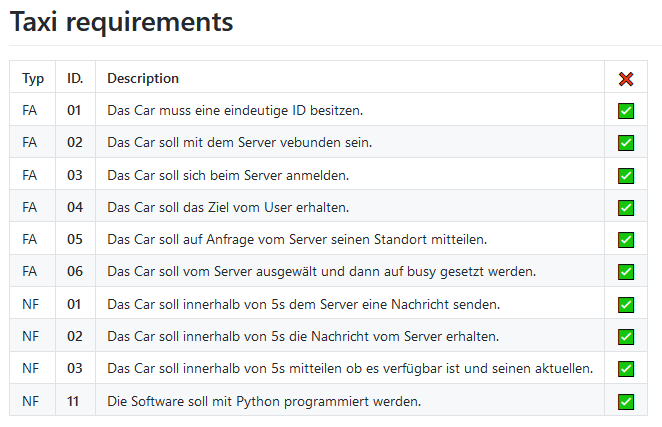
\includegraphics[width=0.48\textwidth]{Bsp_requirments.png}
     \caption{Requirments}
\end{figure}




\subsection{Use-Case}

Der Nächste Schritt im Projekt, ist aus dem gesammelten Informationen der Requirements, Use-Case Diagramme für jeden Client zu erstellen.


Use-Case Diagramme verdeutlichen die 
Aufgaben und 

Verbindungen zwischen den einzelnen Clients.


Vorab Registrieren sich alle Clients beim Server, so ist der Server mit jedem Client verbunden.


Nun bekommt der Server eine Message vom User, 'request car'.
Folgend wird 'select closest car' vom Server durchgeführt und dem nächsten gelegenen Car mitgeteilt, das eine anfragende vom User eingegangen ist.

Zudem sind in der Message die Koordinaten des Users enthalten, woraufhin das Car zu diesem Standort fährt.

Der Server setzt das bestellte Car auf Busy, 'change car status'.


Danach erhält das Car eine Message vom User mit dem gewünschten Zielort und bringt ihn dort hin.


Am Zielort setzt der User dann das Car beim Server wieder auf free.


Zum Schluss erfragt der Server den neuen Standort des Cars und schließt die Handlung damit ab.



\begin{figure}[htbp] 
  \centering
     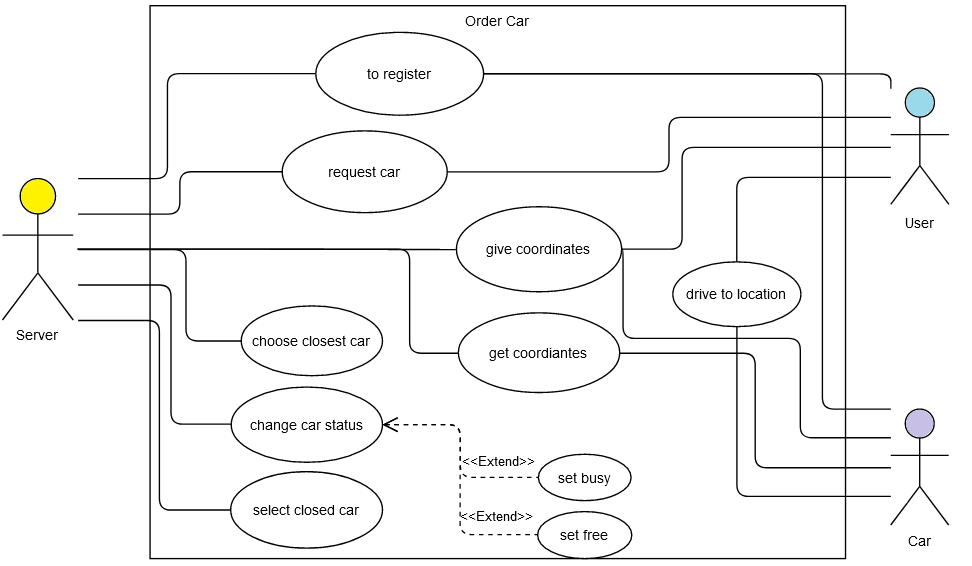
\includegraphics[width=0.48\textwidth]{Use-Case_Server.png}
     \caption{Use-Case}
\end{figure}


